\documentclass{article}
\usepackage{array}
\usepackage{minted}
\usepackage{xcolor}
\usepackage{graphicx}
\graphicspath{{./images/}}
\definecolor{LightGray}{gray}{0.9}
\usemintedstyle{vs}
\title{Software Development Week 3}
\author{Nathan Le Brun}
\date{\today}
\begin{document}
    \maketitle
    VSV Id: 107027
    
    \section{Operators}
        \subsubsection{Table}
            \begin{tabular}{|c|c|c|}
                \hline
                Operator & Type of operator & Operation \\
                \hline
                = & Assignment & assigns a name to a value \\
                \hline
                <> & Comparison & Returns true if the left value does not equal the right value \\
                \hline
                == & Comparison & Returns true if the left value is equal to the right value \\
                \hline
                <= & Comparison & Returns true if the left value is less than or equal to the right value \\
                \hline
                and & Logical & Returns true is the left and right expressions return true \\
                \hline
                * & Arithmetic & Returns the product of the left and right values \\
                \hline
                || & Logical & Returns true if either the left or right value returns true \\
                \hline
                > & Comparison & Returns true if the left value is greater than the right value \\
                \hline
                \&\& & Logical & Returns true is the left and right expressions return true \\
                \hline
                ! & Comparison & Returns true if the right value equals false \\
                \hline
                / & Arithmetic & Returns the result of the left value divided by the right value \\
                \hline
                or & Logical & Returns true if either the left or right value returns true \\
                \hline
                != & Comparison & Returns true if the left value does not equal the right value \\
                \hline
            \end{tabular}
        \subsubsection{Identical Operators}
        The || and OR operators, \&\& and AND,  are identical in practice.
    \section[Data Types]{Data Types}
        \begin{center}
            \begin{tabular}{ | m{4cm} | m{3cm} | m{4cm} | m{3cm} | }
                \hline
                Data to store & Data type & Justification & Variable name \\
                \hline
                Person's age & \verb|Uint| & numerical value, cannot be decimal or negative & \verb|$age| \\
                \hline
                Interest rate & \verb|Float| & Needs to support decimals & \verb|$interest_rate| \\
                \hline
                Person's surname & \verb|String| & Has characters & \verb|$surname| \\
                \hline
                Australian postcode & \verb|Uint| & Cannot be decimal or negative & \verb|$postcode| \\
                \hline
                Australian and international postcodes & Array of String (\verb|String[]|) & List of postcodes, international postcodes can contain letters & \verb|$postcodes| \\
                \hline
                Person's date of birth & \verb|String| & Too many different formats & \verb|$dob| \\
                \hline
                State of a light switch & \verb|Bool| & Can be represented as on or off & \verb|$is_on| \\
                \hline
            \end{tabular}
        \end{center}
    \section{Conditionals}
        \subsubsection{Switch Statement}
            \begin{minted}[breaklines, bgcolor=LightGray]{php}
<?php
  declare(strict_types = 1);
  function select_choice(int $choice): string {
    switch ($choice) {
      case 1:
        return "Here is your lemonade";
        break;
      case 2:
        return "Here is your orange squash";
        break;
      case 3:
        return "Here is your cola";
        break;
      case 4:
        return "Here is your ginger beer";
        break;
      default:
        return "nuh uh";
        break;
    }
  }
?>
            \end{minted}
            \begin{figure}[h]
                \centering
                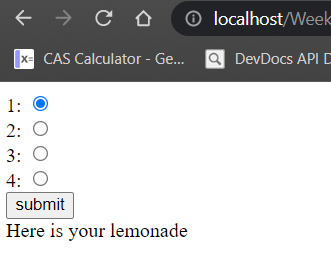
\includegraphics{SwitchOutput}
                \caption{The output of the code shown above}
            \end{figure}
        \subsubsection{If Statements}
            \begin{minted}[breaklines, bgcolor=LightGray]{php}
<?php
  function age_check(int $age): string {
    if ($age < 3) return "You are too young for school";
    if ($age > 18) return "You do not have to go to school";
    if ($age < 5) return "You can go to preschool";
    if ($age < 12) return "You can go to primary school";
    return "You can go to high school";
  }
?>
            \end{minted}
            \begin{figure}[h]
                \centering
                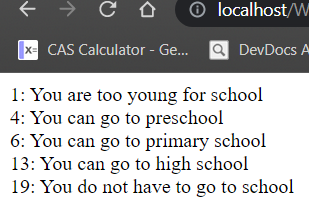
\includegraphics{IfOutput}
                \caption{The output of the code shown above}
            \end{figure}
\end{document}